\chapter{Introduction}

%Provide a short summary of the whole PhD thesis:
% -Introduction to QC & CQED
% -Building Blocks of Superconducting Quantum Processors
% -Realization of a 2-Transmon QP
% -Tune-Up & Characterization of the Universal 2-Qubit Gate
% -Grover's Algorithm: Introduction & Background
% -Implementation on the 2-Qubit Processor
% -Design of a Scalable QC Architecture

\section{Quantum Computing \& Circuit Quantum Electrodynamics}

\begin{figure}
	\centering
		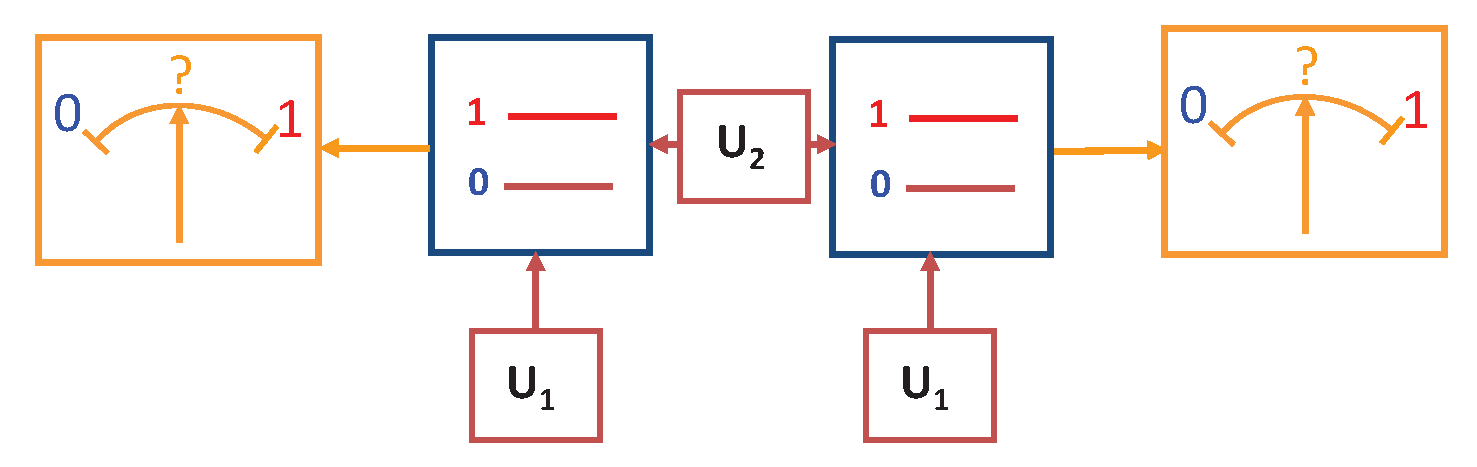
\includegraphics[width=1.\textwidth]{./material/papers/grover/submission1/Fig1}
	\label{fig:Grover1}
	\caption{A blueprint of a 2 qubit quantum processor}
\end{figure}

This thesis presents experiments performed on on superconducting 2-Qubit quantum processor. The main goal of this work was to demonstrate a possible quantum computing architecture using superconducting qubits that follows the canonical blueprint of a 2-qubit quantum processor as formulated by \cite{diVincenzo:Criteria} and as shown in fig. \ref{fig:Grover1}. In this respect, a universal quantum computer is a register of quantum bits -or qubits- on which one can perform universal 1- and 2-qubit quantum gates. In addition, one can read out the state of each qubit individually and with high fidelity and reset the qubit register to a well-defined product state.

Implementing this allegedly simple list of requirements in a system of superconducting qubits has been a major research challenge during the last decade. The first demonstration of coherent quantum-mechanical dynamics in a superconducting structure by \cite{Nakamura} sparked a broad research field about superconducting quantum bits. In the years following Nakamura's discovery, several types of superconducting qubits were proposed and realized, using superconducting phase \cite{PhaseQubits}, magnetic flux \cite{FluxQubits} or electrical charge \cite{ChargeQubits} as the dominant quantum variable. An important milestone was in 2001 the development of the Quantronium qubit at Saclay \cite{Quantronium}, which showed for the first time a coherence time larger than 1 $\mu s$ and made it possible to perform robust, high fidelity single-qubit operations. In 2004, the development of the so called Transmon qubit together with the concept of circuit quantum electrodynamics in Yale \cite{WallraffCQED} marked another important milestone for this research field by drastically simplifying the design of the superconducting qubits and by creating a reliable platform for multi-qubit experiments. Within this approach, simple quantum gates and algorithms with up to four qubits have been implemented, demonstrating multi-qubit entanglement \cite{2QubitEntanglement,3QubitEntanglement} and simple quantum algorithms \cite{Baur,diCarlo}.

In parallel to this, the development of quantum-limited amplifiers based on non-linear superconducting resonators \cite{Siddiqi} complemented the CQED architecture by providing a fast and high-fidelity readout scheme for Transmon qubits \cite{Metcalfe,Mallet} and for the amplification of quantum signals in general. This opened up the road to the direct observation of quantum jumps in superconducting qubits \cite{Siddigi?} and even for implementing simple forms of quantum feedback \cite{Siddiqi}.

Another important recent breakthrough is the development of a qubit architecture using three-dimensional superconducting cavitities instead of one-dimensional coplanar waveguide resonators in the CQED approach \cite{Yale}. Producing an increase in qubit lifetime of one order of magnitude, this technique opened the road to more complex quantum feedback and error correction experiments.

This work wants to fit in this global picture by complementing the CQED approach with a single-shot, individual qubit readout. Such a readout is absolutely necessary when pursuing the long-term goal of a superconducting quantum computer but -up to now- was just not provided by ``classical'' CQED.

\section{Building a Superconducting Quantum Processor}

\subsection{Building Blocks}

\subsection{Simultaneous Single-Shot Qubit Readout}

\subsection{Generation of Entanglement between Qubits}

\subsection{Implementing an Universal 2-Qubit Gate}

\subsection{Running a Quantum Algorithm}

\section{Scaling Up To Multiple Qubits}

\subsection{Principles}

\subsection{Problems}

\subsection{Possible Approaches}

\subsection{Implementation}

\begin{figure}
	\centering
		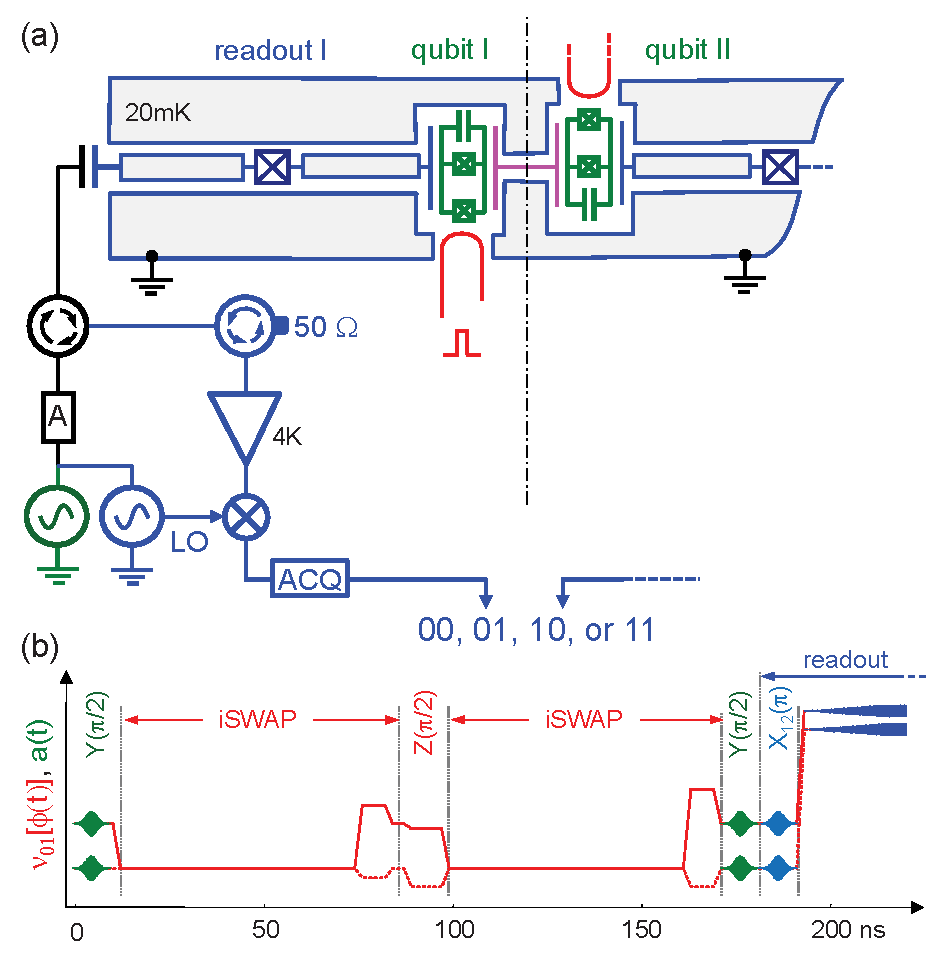
\includegraphics[width=1.\textwidth]{./material/papers/grover/submission1/Fig2}
	\label{fig:Grover2}
	\caption{}
\end{figure}

\begin{figure}
	\centering
		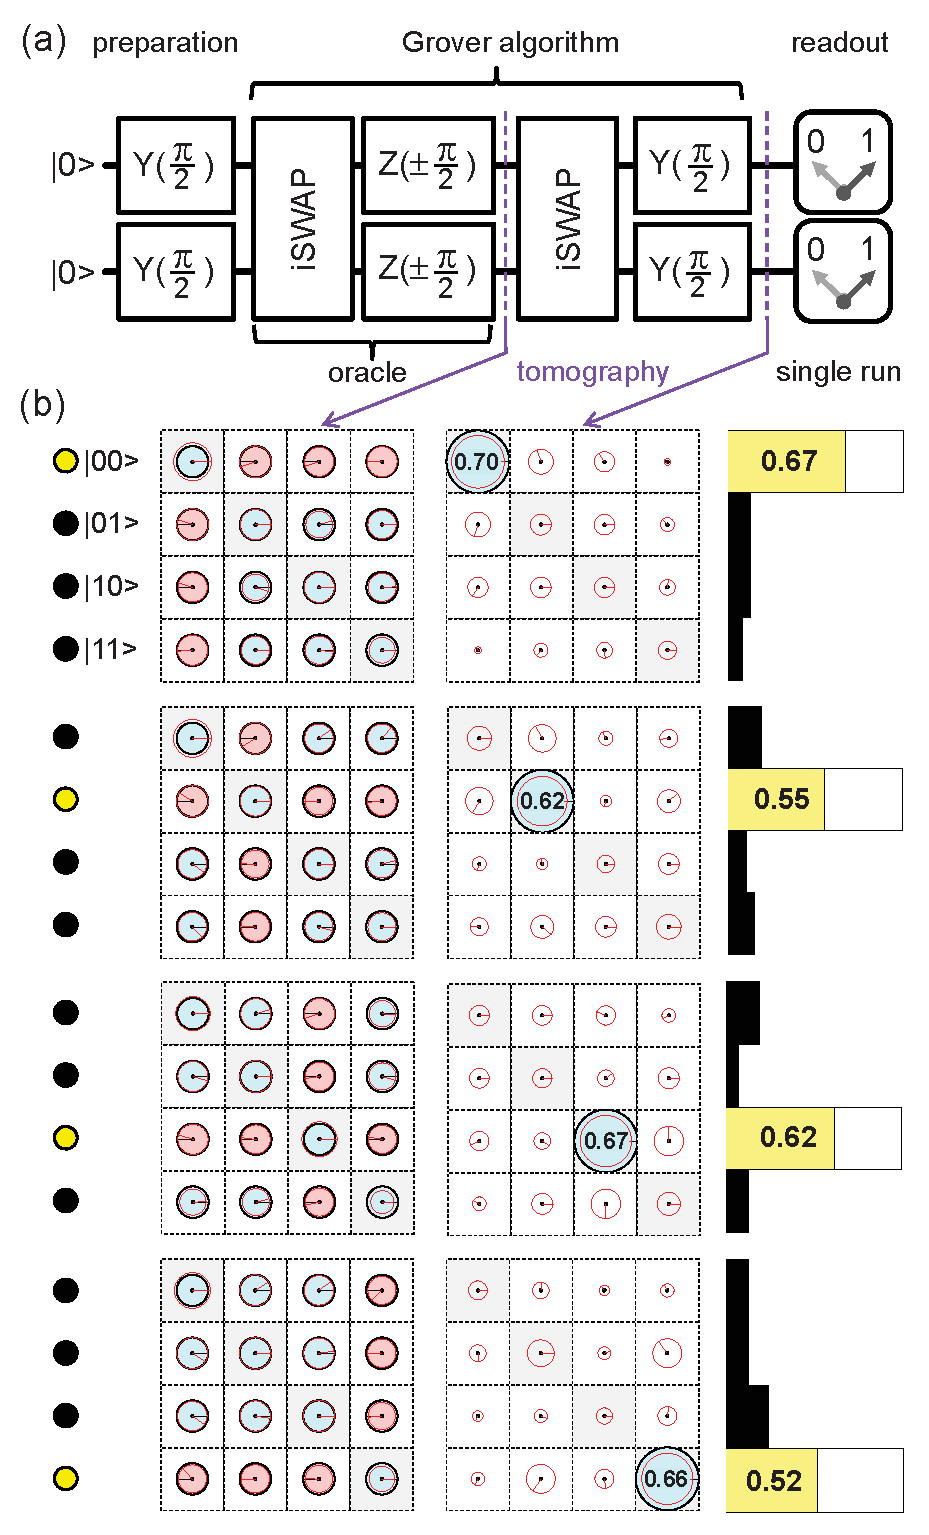
\includegraphics[width=1.\textwidth]{./material/papers/grover/submission1/Fig3}
	\label{fig:Grover3}
	\caption{}
\end{figure}


%2 Qubit Paper Figures

\begin{figure}
	\centering
		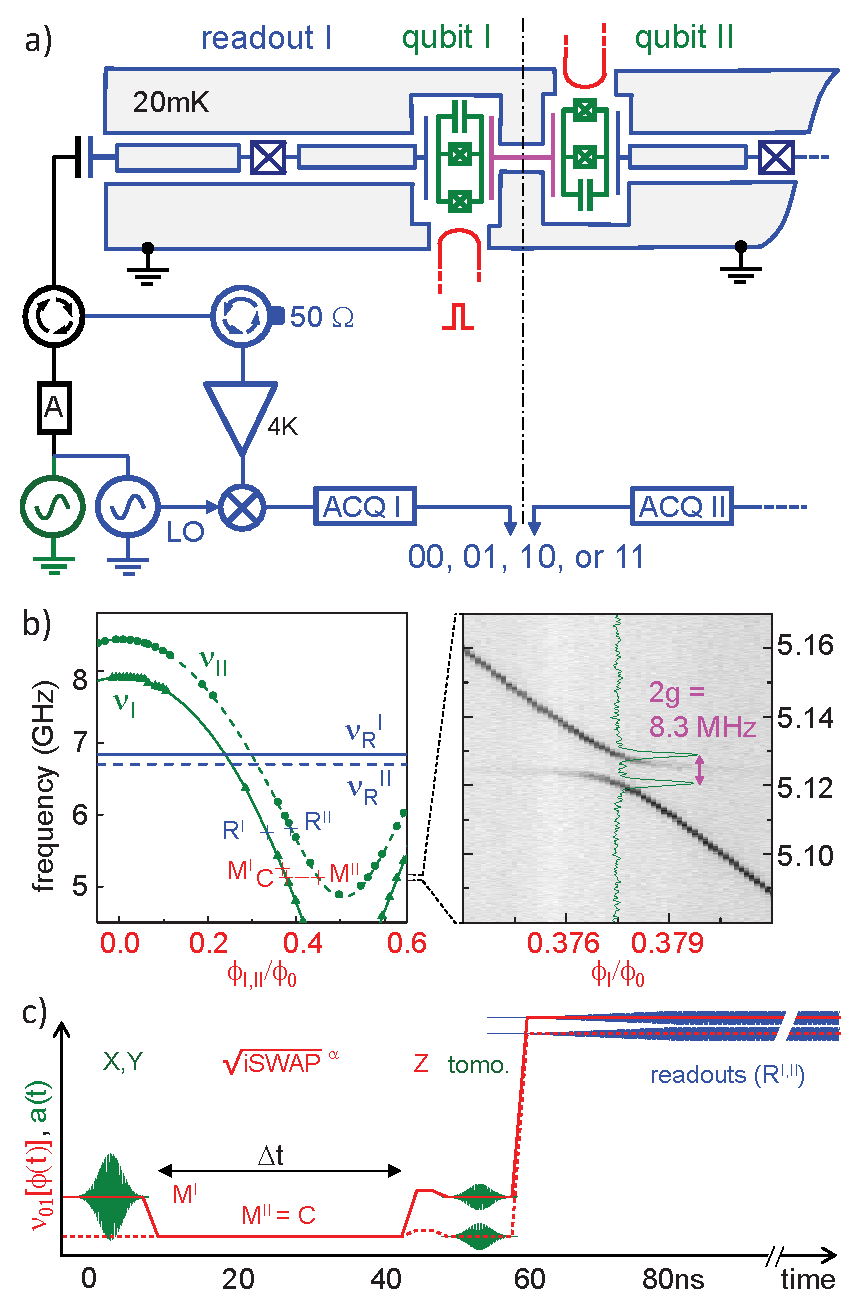
\includegraphics[width=1.\textwidth]{./material/papers/iswap/submission1/Dewes_Figure1}
	\label{fig:iSwap1}
	\caption{}
\end{figure}

\begin{figure}
	\centering
		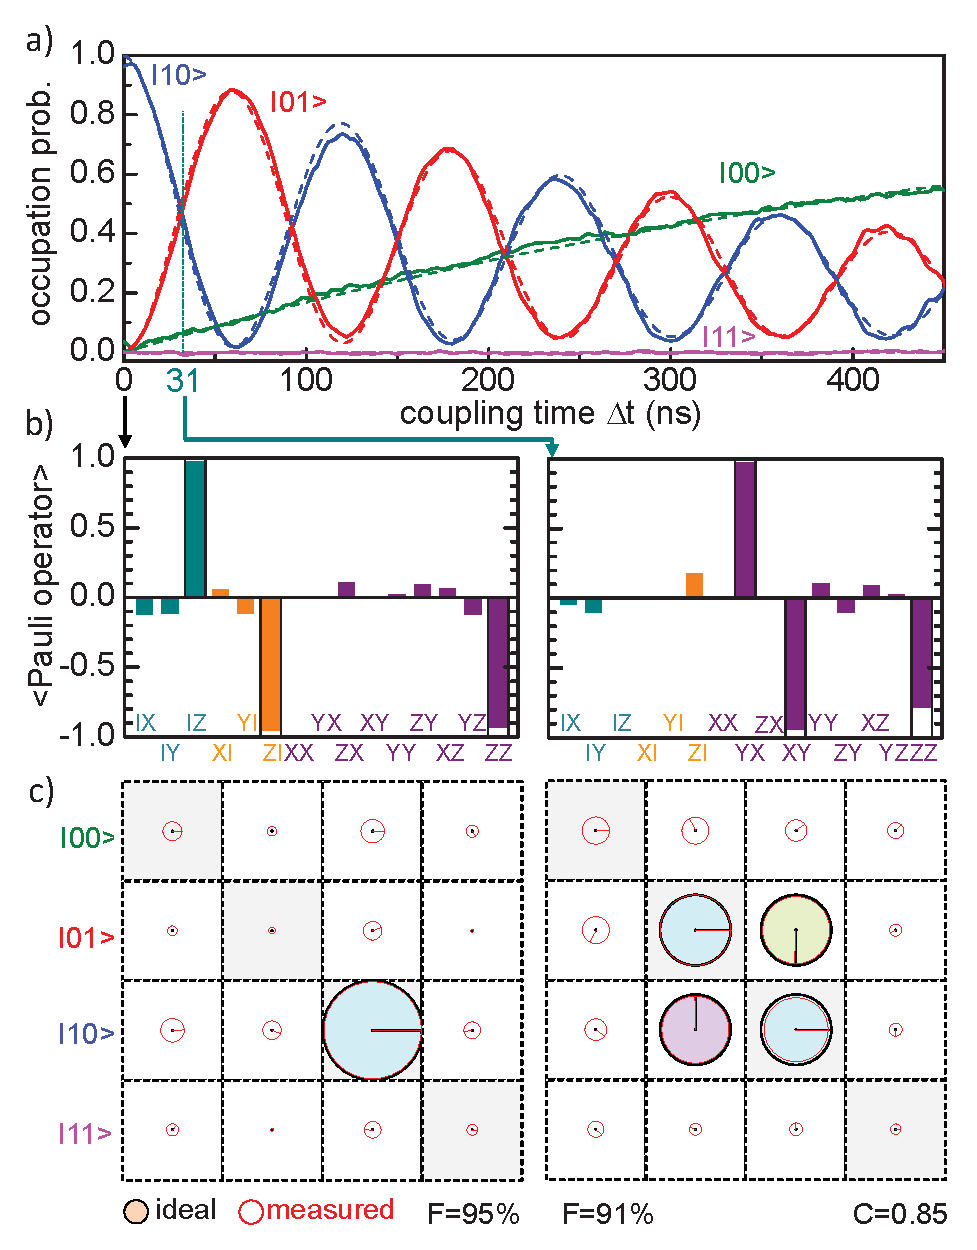
\includegraphics[width=1.\textwidth]{./material/papers/iswap/submission1/Dewes_Figure2}
	\label{fig:iSwap2}
	\caption{A blueprint of a 2 qubit quantum processor}
\end{figure}

\begin{figure}
	\centering
		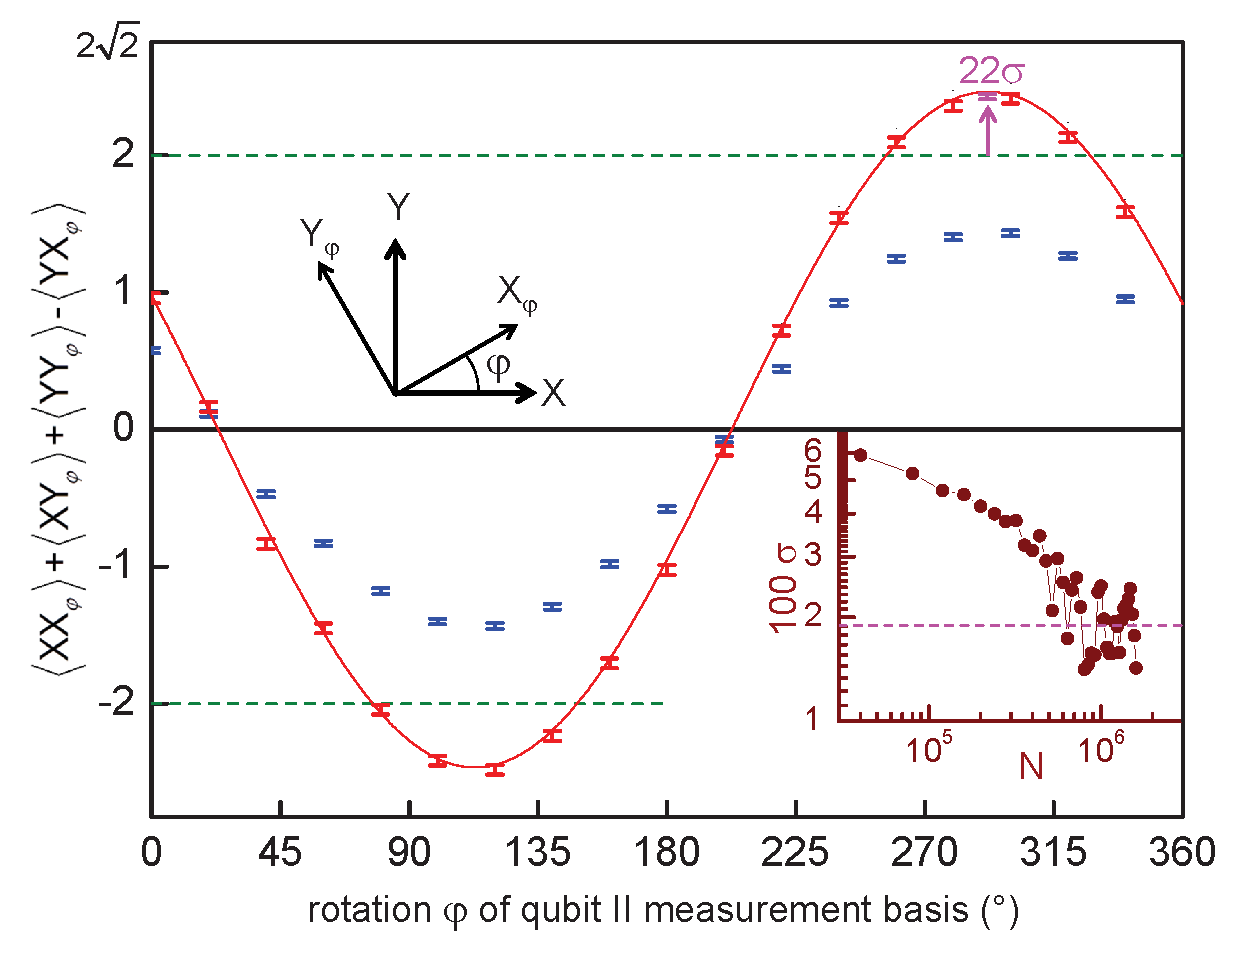
\includegraphics[width=1.\textwidth]{./material/papers/iswap/submission1/Dewes_Figure3}
	\label{fig:iSwap3}
	\caption{}
\end{figure}

\begin{figure}
	\centering
		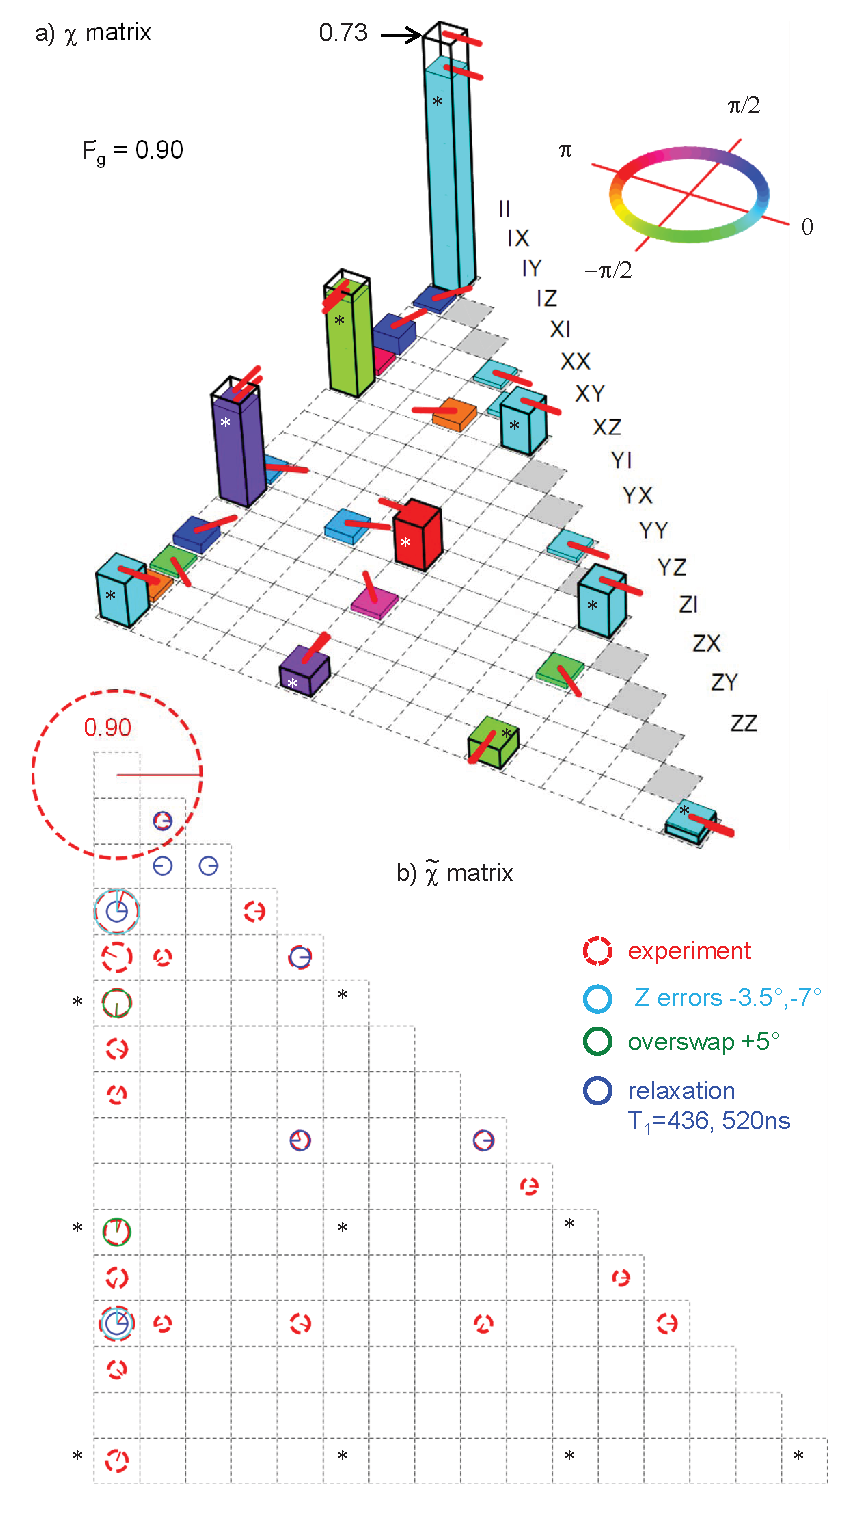
\includegraphics[width=1.\textwidth]{./material/papers/iswap/submission1/Dewes_Figure4}
	\label{fig:iSwap4}
	\caption{}
\end{figure}
